\chapter{Gleichzeitigkeit}\label{cha:gleichzeitigkeit}

\section{Einleitung}
Probleme der Gleichzeitigkeit entstehen immer dann, wenn mehrere Benutzer oder Prozesse zeitgleich auf eine Datenbank zugreifen können. Das DBMS muss hierbei einen Kontrollmechanismus bereitstellen, der gewährleistet, dass keine inkonsistenten Zustände auftreten.

\section{Transaktionen}
\begin{figure}[H]
\centering
    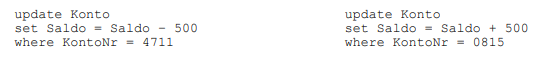
\includegraphics[width=.75\textwidth]{Content/images/gleichzeitigkeit/banktransaktion.png}
    \caption{Beispiel Banktransaktion}
\end{figure}
\noindent
Bei einer Banküberweisung muss sichergestellt werden, dass sowohl die Abbuchung, als auch die Gegenbuchung stattfinden. Wird nur eines der Statements durchgeführt, so gerät die Datenbank in einen inkonsistenten Zustand. Die Buchungen werden daher in einer Transaktion zusammengefasst. Eine Transaktion ist eine logisch zusammenhängende Sequenz von Operationen, die eine Datenbank von einem konsistenten Zustand in einen anderen konsistenten Zustand überführt. Sie darf nur in ihrer Gesamtheit durchgeführt werden.  Schlägt eine der Teiltransaktionen in der Gruppe fehl, werden alle anderen Teilaktionen ebenfalls rückgängig gemacht (Rollback). Transaktionen verhindern, dass die Datenbank in einen inkonsistenten Zustand gerät, wenn ein Problem bei der Durchführung einer der Aktionen auftritt, aus denen sich die Transaktion zusammensetzt.

\subsection{Die ACID-Eigenschaften von Transaktionen}
Bei einer Transaktion muss das Transaktionssystem die ACID-Eigenschaften garantieren und beherrschen:

\subsubsection*{Atomarität}
Eine Transaktion wird vollständig oder gar nicht ausgeführt. Die Transaktion ist unteilbar und wenn Sie abgebrochen wird, hat das keine Auswirkungen auf das System.

\subsubsection*{Konsistenz}
Nach einer Ausübung einer Transaktion muss der Datenbestand wieder konsistent sein und darf keine Anomalien aufweisen.

\subsubsection*{Isolation}
Jede Transaktion arbeitet unabhängig von anderen Transaktionen. Gleichzeitige Transaktionen dürfen sich gegenseitig nicht beeinflussen.

\subsubsection*{Dauerhaftigkeit}
Wenn eine Transaktion die Datenbasis verändert, so gilt diese Änderung anschließend auf Dauer (persistent, permanent).

\section{Probleme der Gleichzeitigkeit}

\subsection{Lost Update}
\begin{figure}[H]
\centering
    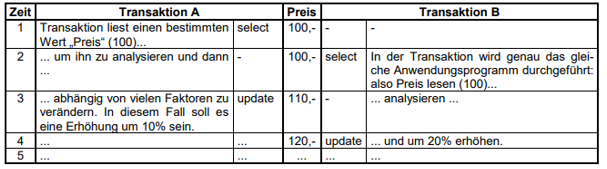
\includegraphics[width=.75\textwidth]{Content/images/gleichzeitigkeit/lostupdate.png}
    \caption{Lost Update}
\end{figure}
\noindent
Transaktion A liest einen bestimmten Datensatz. Transaktion B liest denselben Datensatz noch bevor Transaktion A ihn verändert. Sobald Transaktion B den Datensatz ebenfalls verändert, geht die Veränderung von Transaktion A verloren. Sie ist ein Lost Update.

\subsection{Umcommitted Dependency}
\begin{figure}[H]
\centering
    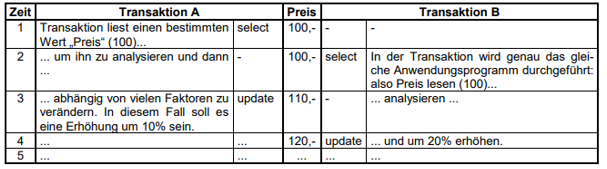
\includegraphics[width=.75\textwidth]{Content/images/gleichzeitigkeit/lostupdate.png}
    \caption{Umcommitted Dependency}
\end{figure}
\noindent
Transaktion A verändert einen Wert, der im Anschluss wieder zurück gerollt wird. Transaktion B liest der Wert noch vor dem Rollback und rechnet mit dem veränderten Wert. 
Das Problem der Uncommitted Dependency tritt dann auf, wenn eine Transaktion mit einem Wert rechnet der verändert, aber noch nicht committed wurde. Man spricht auf von einem „dirty read“, also vom Lesen, vor der Änderungsbestätigung. 

\subsection{Inconsistent Analysis}
\begin{figure}[H]
\centering
    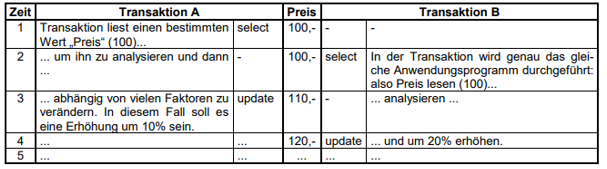
\includegraphics[width=.75\textwidth]{Content/images/gleichzeitigkeit/lostupdate.png}
    \caption{Inconsistent Analysis}
\end{figure}
\noindent
Eine inconsistent Analysis tritt dann auf, wenn eine Transaktion Werte liest und analysiert, die von einer anderen Transaktion verändert werden. Dabei kann es auch zum Phantom-Problem kommen: Die Menge der zu lesenden Objekte werden durch INSERTs / DELETs verändert.

\section{Locking}
Um die Probleme der Gleichzeitigkeit zu verhindern, werden Objekte gesperrt (gelockt). Eine solche Sperre ermöglicht den exklusiven Zugriff eines Prozesses auf eine Ressource, d. h. mit der Garantie, dass kein anderer Prozess diese Ressource liest oder verändert, solange die Sperre besteht. 

\subsection{Locking-Arten}
\subsubsection*{Exclusive Lock (X-Lock, Write-Lock)}
Eine Ressource mit einem Exclusive Lock verhindert, dass die Ressource von anderen Prozessen gelesen oder geschrieben wird, da der Prozess, der den Lock gesetzt hat, die Ressource verändern möchte. Das Verfahren wird auch als pessimistisches Locking bezeichnet, da es von der Annahme ausgeht, dass in der Regel eine Aktualisierung der Daten erfolgen wird. Beim optimistischen Locking wird davon ausgegangen, dass in der Regel keine Aktualisierung erfolgt oder eine gleichzeitige Aktualisierung durch zwei Nutzer nicht wahrscheinlich ist. Es wird erst beim Aktualisieren geprüft, ob der Wert verändert wurde.

\subsubsection*{Shared Lock (S-Lock, Read-Lock)}
Besitzt eine Ressource einen Shared Lock, so möchte der Prozess, der diese Sperre gesetzt hat, von der Ressource nur lesen. Somit können auch andere Prozesse auf diese Ressource lesend zugreifen, dürfen diese aber nicht verändern.
\newline
\newline
Mithilfe von Locking werden die Probleme der Gleichzeitigkeit gelöst:
\begin{itemize}
    \item Lost Update: Transaktion B bekommt das Schreibrecht erst, wenn Transaktion A die Veränderung vorgenommen hat.
    \item Uncommitted Dependency: Transaktion B bekommt das Leserecht erst, nachdem Transaktion A zurück gerollt wird.
    \item Inconsistent Analysis: Transaktion B bekommt das Schreibrecht erst, wenn Transaktion A mit der Analyse fertig ist.
\end{itemize}

\subsection{Deadlocks \& Strategien zur Vermeidung}
Das Setzen einer Sperre kann Deadlocks verursachen, nämlich dann, wenn zwei Prozesse gegenseitig auf die Freigabe der vom jeweils anderen gesperrten Ressource warten.

\subsubsection{Two Phase Locking}
\begin{figure}[H]
\centering
    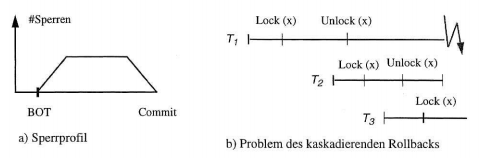
\includegraphics[width=.75\textwidth]{Content/images/gleichzeitigkeit/twophaselocking.png}
    \caption{Inconsistent Analysis}
\end{figure}
\noindent
Das 2-Phasen-Sperrprotokoll ist das gängigste Sperrverfahren und wird in zwei Varianten unterschieden. Die Gemeinsamkeit besteht darin, dass eine Transaktion nach bestimmten Regeln, sogenannten Protokollen abgearbeitet wird.
Die zwei Phasen des Protokolls bestehen aus einer Sperrphase, in der alle benötigten Objekte für die Transaktion gesperrt werden. In der zweiten Phase werden die Sperren wieder freigegeben, sodass die Objekte von anderen Transaktionen genutzt werden können.  
\newline
\newline
Wird nun aber eine Transaktion  (aus irgendwelchen Gründen) abgebrochen und zurückgerollt, so müssen auch die später durchgeführten Transaktionen kaskadierend zurückgerollt werden.

\begin{minipage}{0.4\textwidth}
\begin{figure}[H]
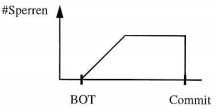
\includegraphics{Content/images/gleichzeitigkeit/striktezweiphasigkeit.png}
\end{figure}
\end{minipage} \hfill
\begin{minipage}{0.55\textwidth}
\paragraph{Strikte Zweiphasigkeit}
Durch eine strikte Zweiphasigkeit werden alle Sperren erst am Ende einer Transaktion freigegeben. Dadurch kann eine Transaktion ohne Auswirkungen auf andere Transaktionen abgebrochen werden. Ein fortgepflanzter Rollback kann nicht eintreten.
\end{minipage}

\begin{minipage}{0.4\textwidth}
\begin{figure}[H]
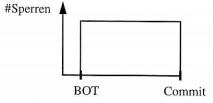
\includegraphics{Content/images/gleichzeitigkeit/preclaiming.png}
\end{figure}
\end{minipage} \hfill
\begin{minipage}{0.55\textwidth}
\paragraph{Preclaiming}
Mit dem Preclaiming werden zu Beginn einer Transaktion alle Objekte gesperrt. Dadurch werden Deadlocks oder Abbrüche durch andere Transaktionen verhindert. Die Schwierigkeit besteht jedoch darin, dass es sehr aufwändig ist, bereits vor einer Transaktion alle benötigten Objekte zu kennen und zu sperren. Preclaiming ist daher für die Praxis nicht relevant.
\end{minipage}

\subsubsection{Transaktions-Scheduling}
Dieses Verfahren beschränkt die parallele Durchführung: nur solche Transaktionen dürfen sich zeitlich überlappen, die keine gemeinsamen Datenobjekte behandeln. Damit behindern sich die Transaktionen gegenseitig niemals.
\newline
Voraussetzung ist, dass bereits vor dem Ausführen der Operationen bekannt ist, auf welche Datenobjekte zugegriffen wird. Da man dies i.a. nicht „sagen“ bzw. automatisch feststellen kann, sind solche Verfahren pessimistisch: es werden daher oft unnötigerweise Transaktionen von der Verarbeitung ausgeschlossen.

\subsubsection{Zeitmarken-Verfahren}
Die Grundidee dabei ist, dass jede Transaktion einen Zeitstempel (timestamp) zur eindeutigen Identifikation erhält. Diese Zeitmarke (= Transaktions-Startzeitpunkt) ordnet der Transaktion gleichzeitig eine bestimmte Priorität zu: je älter oder jünger eine Transaktion ist, desto eher kommt sie zum Zuge. Konflikte werden nach einem genau definierten Schema durch eine Kombination aus Warten (Wait) und Restart (Rollback and Retry) jeweils einer der im Konflikt befindlichen Transaktion gelöst.
\newline
Wenn die Transaktion A einen von B bereits gesperrten Datensatz sperren will, dann passiert je nach gewähltem Verfahren folgendes:
\begin{itemize}
    \item \textbf{Wait-Die:} Falls A älter ist als B, wartet A sonst (falls A jünger als B) wird A zurückgenommen
    \item \textbf{Wound-Wait:} Falls A älter ist als B, wird B zurückgenommen sonst (falls A jünger als B) wartet A
\end{itemize}

\subsubsection{Timeout}
Eine weitere recht gebräuchliche Methode ist die Angabe eines sogenannten Time-Outs: auch hier wird für jede Transaktion vermerkt, wann sie gestartet wurde. Ist sie nach einer bestimmten, als Systemparameter einstellbarer Dauer nicht beendet, so wird angenommen, dass sie in einem Deadlock steckt – sie wird zurückgenommen.

\section{Serialisierbarkeit}
In Transaktionssystemen existiert ein Ausführungsplan für die parallele Ausführung mehrerer Transaktionen. Der Plan wird auch Historie genannt und gibt an, in welcher Reihenfolge die einzelnen Operationen der Transaktion ausgeführt werden. Als serialisierbar wird eine Historie bezeichnet, wenn sie zum selben Ergebnis führt wie eine nacheinander (seriell) ausgeführte Historie über dieselben Transaktionen. Überprüft werden kann die Serialisierbarkeit mithilfe eines Precedence Graphs.

\subsection{Precedence Graph}
Eine Menge von Datenbank-Transaktionen lässt sich genau dann serialisieren, wenn der zugehörige Serialisierbarkeitsgraph zyklenfrei ist.
\subsubsection*{Relegn für das Zeichnen}
\begin{itemize}
    \item Transaktionen werden durch Knoten dargestellt
    \item Pfeile zwischen Knoten für:
    \begin{itemize}
        \item R1(A) $\longrightarrow$ W2(A)
        \item W1(A) $\longrightarrow$ W2(A)
        \item W1(A) $\longrightarrow$ R2(A)
    \end{itemize}
\end{itemize}

\subsubsection*{Beispiel 1 - serialisierbar}
\begin{figure}[H]
\centering
    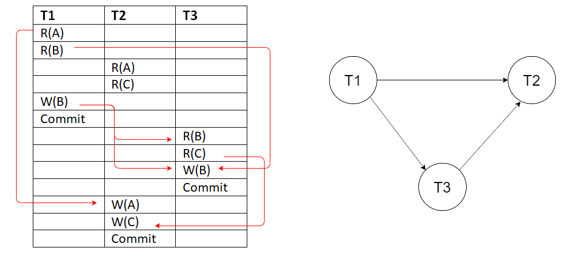
\includegraphics[scale=1.0]{Content/images/gleichzeitigkeit/example1.png}
\end{figure}

\subsubsection*{Beispiel 2 - nicht serialisierbar}
\begin{figure}[H]
\centering
    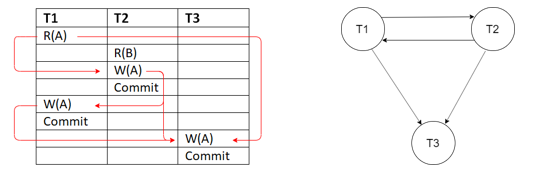
\includegraphics[scale=1.0]{Content/images/gleichzeitigkeit/example2.png}
\end{figure}

\section{Anhang Prof. Kainerstorfer}
\subsection*{Wie prüft man einen Schedule auf Deadlocks?}
Man stellt die einzelnen Logs auf und prüft den Wartegraphen. Ein Log ist eine Folge von Transaktionen auf ein bestimmtes Objekt. Folgendes Beispiel soll das Vorgehen erläutern.

\subsubsection*{Folgender Schedule ist gegeben:}
\textbf{S[r1(b),r2(b),w2(b),r2(c),r2(d),r3(b),r4(d),w3(a),w4(d),r5(a),r5(c),w2(c)]}

\subsubsection*{Aufstellen der Logs für die beteiligten Objekte a,b,c und d}
\begin{center}
\begin{tabular}{| c | c | c | c |}
    \hline
    log(a) & log(b) & log(c) & log(d) \\
    \hline
    w3 & r1 & r2 & r2 \\
    r5 & r2 & r5 & r4 \\
     & w2 & w2 & w4 \\
     & r3 &  &  \\
    \hline
\end{tabular}
\end{center}

\subsubsection*{Den Wartegraphen nach dem extrahierten Log aufstellen}
\begin{itemize}
    \item Zeichne für jede Transaktion einen Knoten
    \item Wiederhole für jeden Log in welchem mindestens eine Transaktion schreibt und zwei lesend zugreifen
    \begin{itemize}
        \item Verbinde jede Leseoperation r vor dem Write mit dem Knoten der Schreibertransaktion
        \item Verbinde jede Schreibertransaktion mit jedem danach folgenden Readbefehl
        \item Schlingen sind zwecklos und können dabei ignoriert werden
    \end{itemize}
\end{itemize}
\begin{figure}[H]
\centering
    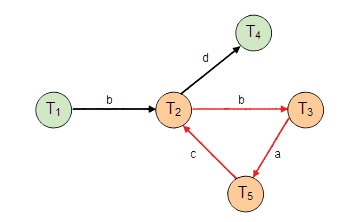
\includegraphics[scale=1.0]{Content/images/gleichzeitigkeit/example3.png}
\end{figure}
\subsubsection*{Wartegraph auf Zyklus prüfen, denn mit ist der Schedule nicht serialisierbar}
Wie wir sehen enthält der Graph einen Zyklus. Dies bedeutet, daß die genannten Bedingungen in den Logs nicht gelten. Und zwar das die Reihenfolgen der Zugriffe in allen Logs gleich ist. Dies ist hier nicht der Fall. Denn was nicht sein darf, ist
\newline
\textbf{T2 vor T3 kommt, T3 vor T5 komt und T5 vor T2 kommt}
\newline
Deshalb erzeugen T2, T3 und T5 einen Deadlock.
